\chapter{Technology Review}

\section{GitHub}
GitHub is a Version Control Software that stores the entire code history of projects in what they call 'Repositories' (Figure 3.1), with READMEs and Wikis in Markdown for documentation. Repositories can be used for individual usage, and they can add collaborators to commit (contribute) to the repository. For team-based usage, an organization can be created that would contain individual repositories that all team members can commit to the repository. It is an amazing tool. With GitHub, if something went wrong with a project, e.g. a bug or a sudden loss of files, they can all be recovered from the repository making it easier and faster to fix problems. It gives the opportunity to show off work their users have done to future employers without having to send ZIP files or screenshots. GitHub was widely used in this project, from the repository to the projects board, Wikis and the issues.

\begin{figure}[H]
    \caption{Repota App Repository}
    \label{image:gitRepo}
    \centering
    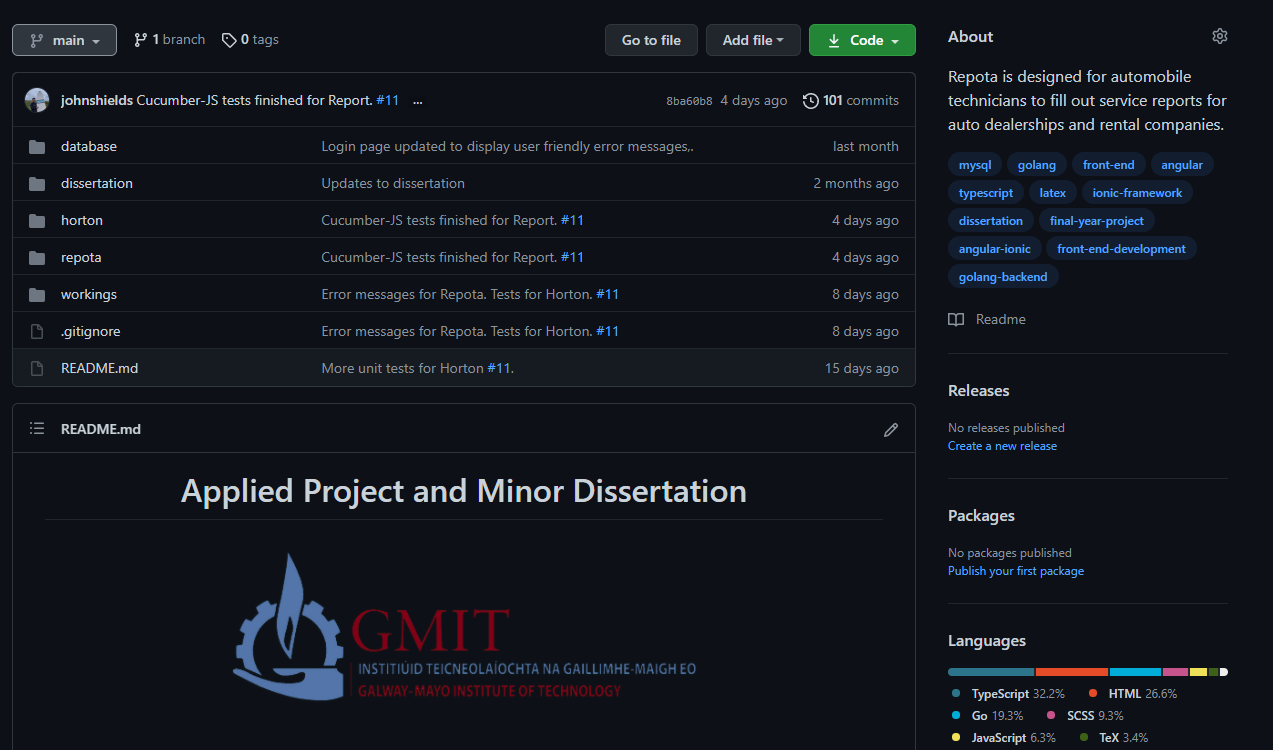
\includegraphics[width=0.7\textwidth]{images/misc/git-repo.png}
\end{figure}

\section{OpenAPI}
OpenAPI specification are machine-readable API blueprints for RESTful web services. Client and Server stubs can be generated along with documentation just from these blueprints. OpenAPI enables to perfect with an efficiency of design and testing. Swagger Tools by Smart Bear allow for the implementation of specifications for these blueprints. These blueprints can be written in a human and machine-readable format of YAML. They can also be written in JSON.  YAML is almost living documentation of an API, whereas JSON may take a longer time to understand as it is more focused towards machines. \cite{ref6}

\subsection{API Specification}
As said above, an API Specification (spec) works as a blueprint. API specs are broken down into individual parts. The spec always starts with the version of the OpenAPI, followed by a title, description and a version of the API itself as documentation of the spec. The API's base URL (e.g., - /api/v1/) is then defined under the servers section as an URL. The spec is then broken down into paths that are split into a request and a response. The path's request part includes; a HTTP method such as POST, a description of what the path can do, an operationId as a unique identifier for the method (handler function), a request body of a schema model with an example of data objects and any security that is required to make the request to the path such as an API key or a cookie. The response part entails the possible status code and message such as a 200 for success, 400 for a bad request and 500 for internal server errors. Schema models can also be defined within a spec. Schema models contain the following properties; the identifier, name, description and the data fields, types and values. These models represent request payloads to POST/send data to a server in request bodies. \cite{ref6}

\subsection{How OpenAPI fitted the API's design}
Swagger Tools was highly used for prototyping the project's, server and client API stubs along with their data models that resembled the data in the project's database. With Swagger, from OpenAPI specs, server stubs can be easily designed with the necessary paths, HTTP methods, handler functions and response status codes and messages. To follow the server's stubs, the client stubs can be generated with the integrated design to allow the client to talk back and forth to the server. Swagger made the process of designing the project's OpenAPI specification a structured and straightforward task. It proved to be extremely useful to design an API efficiently especially with the specification's documentation and an easy to use tool for a first-time user.

\section{Golang}
Golang (Go), designed by Google, is inspired by the style of Object-Oriented Programming (OOP) Languages. Go is a relatively new language (first version released on November 10, 2009), open-source and becoming widely used. Go is primarily based on the C programming language and has compile speeds that can be as fast as Java and C++ \cite{ref7}. Figure 3.4 is from an article that compared the languages Java, C++ and Go. Go's creators desired the security and performance of Java and C++, but with the "lightness and fun" of a dynamically typed interpreted language such as Python. Go's syntax is influenced by C with a mixture of Pascal. \cite{ref8}
When it comes to OOP, Go is especially great for refactoring and abstraction. Go does not use classes like Java does; the closest element to a class in Go is a Struct that can be used for object-like data models. \cite{ref9} Go files (controllers) can easily pick up functions from others as long as they are in the same package. A function can be abstracted from one controller, put into another, and still be called from in the original controller with no changes or additions. If a function is in another package, it can easily be used outside with an import of that package and a variable declaring that function. Go also employs encapsulation with localized fields inside packages and they are not exported to others. The remainder capitalized fields, methods and functions are public to all packages. \cite{ref9}

\begin{figure}[H]
    \caption{Go VS Java \& C++ \cite{ref7}}
    \label{image:goJavaCpp}
    \centering
    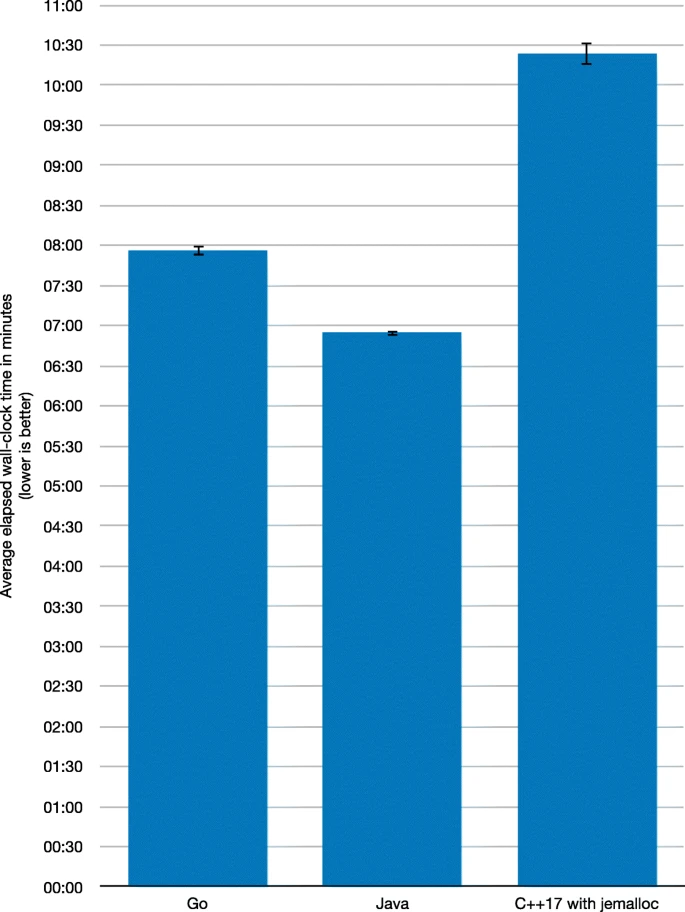
\includegraphics[width=0.5\textwidth]{images/misc/go-java-cpp.png}
\end{figure}

The main idea of Go is to reduce the development of large servers with big machines, many cores, and developers and bring it down to the use of simple tools that can do all those jobs. \cite{ref10} Identifying problems in Go is a more straightforward process as the tools are simple, allowing concentrating on the problem rather than how to solve it. With the Go SDK installation (Software Development Kit), Go's documentation can be obtained from the CLI (Command Line Interface) with the command 'go doc'. For example, simply typing the command 'go doc fmt' into the CLI lists all the documentation on formatting print statements (Figure 3.4). Go doc can also list all the functions inside a project's package (Figure 3.5). With the command 'godoc -http=:6060', a localhost of Go's complete documentation can be accessed, which would provide great use if there is a weak/no internet connection.

\begin{figure}[H]
    \caption{CLI Go Docs on fmt}
    \label{image:goDocFmt}
    \centering
    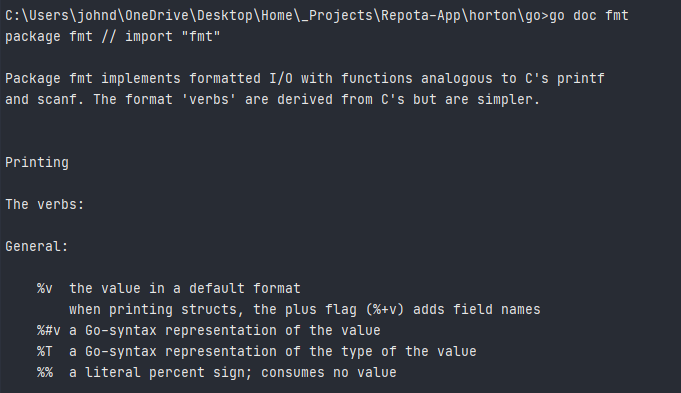
\includegraphics[width=0.8\textwidth]{images/misc/go-doc-fmt.png}
\end{figure}

\begin{figure}[H]
    \caption{Go Functions inside the Back-end's openapi Package}
    \label{image:goFuncs}
    \centering
    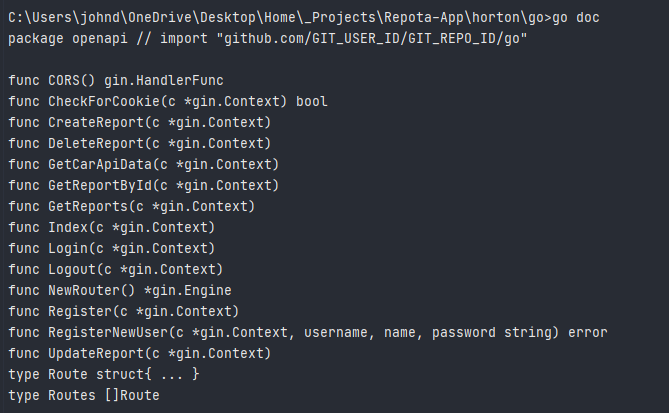
\includegraphics[width=0.8\textwidth]{images/misc/godoc-funcs.png}
\end{figure}

\subsection{Go Web Frameworks}
\subsubsection{Gorilla Mux}
Gorilla Mux is a package that implements the combination of a request router and dispatcher for assigning incoming requests to the designated handler. Mux stands for "HTTP request multiplexer" which is used for incoming HTTP requests are compared to a list of the registered routes and the path that meets the URL or other requirements such as a datatype ID for accessing a complete source of data by its unique identifier. \cite{ref11}

\subsubsection{Gin Gonic}
Gin Gonic has a Martini-like API but with an efficiency that is said to be 40 times faster than Martini. Martini is another Go web framework, which is no longer maintained. Gin is fast with its "Radix tree-based routing, small memory footprint. No reflection. Predictable API performance." \cite{ref12} A chain of middle-wares can handle incoming HTTP requests. Gin's error management makes it simple to gather all of the errors from responses during a HTTP search. Gin allows the creation of custom HTTP response errors (Figure 3.7). Gin needs to be set as a parameter of a function to respond with these errors to implement these custom errors. Suppose a panic occurs in an HTTP request. In that case, Gin can recover it, making it "Crash-free". \cite{ref12} Also, according to an 'Expert analysis' from a JetBrains, GoLand Blog by Ekaterina Zharova, 41\% of Go developers use Gin as their main framework for back-end development. \cite{ref13} Making it the de facto of Go's web frameworks.
\\\\ When an API requires endpoints to share a common path, there is a limitation with Gin. For example 'api/movies/:movieId' and 'api/movies/:releaseDate' will result in a issue with Gin. Having colliding paths in APIs is common, and they can usually switch over and back, but with Gin, they can not. However, depending on the paths required for an API, if the paths are for basic CRUD operations (CREATE, READ, UPDATE AND DELETE), this should not be much of an issue. It becomes an issue when an API needs multiple operations other than CRUD which, Gin does not meet the requirements. For example, a search box on an app would be limited to just one data field, limiting users' convenience. On top of that, it limits the 'RESTfulness' of an API.

\begin{figure}[H]
    \caption{Gin Error Handling}
    \label{image:ginError}
    \centering
    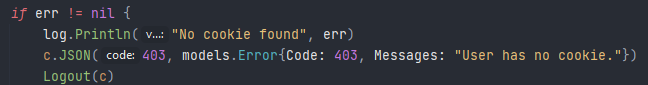
\includegraphics[width=1.0\textwidth]{images/misc/cookie-error.png}
\end{figure}

\subsection{How Go fitted the Back-end}
Back-ends can be developed in many languages, including Java, Python, Ruby, Node.js, and Rust. Go stood out from the others for the back-end for how it handles compile times, syntax, documentation, its use of OOP, and it seemed like a great language to know to expand development skills. 

Learning Go for the first time for the back-end was a welcome challenge. It took some time to become comfortable, and the use of 'go doc' made that process smooth. An element of this challenge was finding a suitable Web Framework that had all the requirements needed. Gorilla Mux was used for the initial setup but failed to effectually meet the requirements to deal with cross-origin issues of HTTP methods for every route with the front-end.
Gin Gonic proved to be the best framework to use, but it required Docker to generate the OpenAPI's server stubs rather than Swagger's standard options. After finalizing the back-end, it can be said that Go is a very nice language to know as it is quite object-oriented and has efficient compile times. 
 
\section{Angular \& Ionic}
There are many JavaScript/TypeScript frameworks out in the web development world, including Angular, React, Vue.js, Meteor and Ember.js. These technologies are primarily JavaScript frameworks. A new JavaScript framework appears almost every year. Some of these frameworks can become obsolete as there is always a new one coming right around the corner.

Angular is a TypeScript-based framework for User Interfaces (UI) that has stayed on the market throughout the years \cite{ref14} and with the combination of Ionic, can make web apps into mobile apps. Also, similar to Go, it was developed by Google after its predecessor AngularJS. Angular has a mighty CLI, which can generate a whole template of an app with routing, testing, and a MVVM (Model-View-ViewModel) for each component. Also, with the CLI, a complete app can be built for production, which translates all the app's code into JavaScript.

Angular is relatively slow to initially compile apps, which is understandable as apps can contain many pages. However, they can be updated once they are up and running without having to rerun them. Angular apps are created with components, and Ionic turns them into pages. Figure 3.8 shows the structure of a page. There are a lot of benefits of using Angular to build apps such as routing, components and it's built in ngIf, ngFor and ngOnInit, which the following subsections will go into detail.

\begin{figure}[H]
    \caption{Angular \& Ionic Home Page Structure}
    \label{image:ngHomePage}
    \centering
    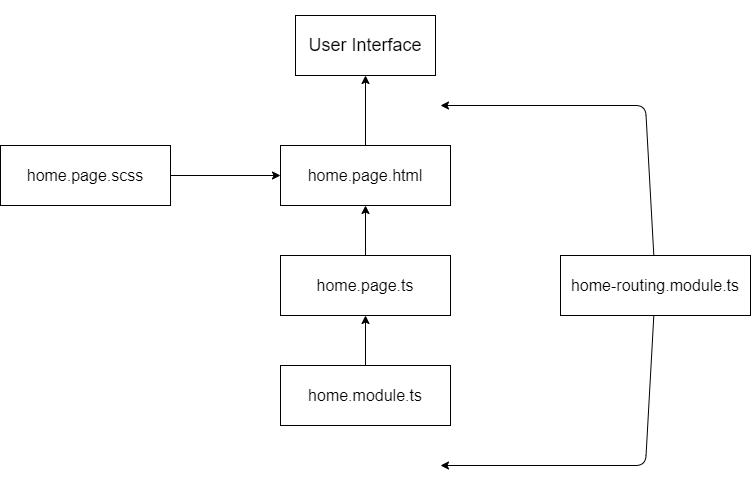
\includegraphics[width=0.8\textwidth]{images/misc/ng-homepage.png}
\end{figure}

\textbf{UI Structure and Styling}
\begin{itemize}
    \item home.page.html \& home.page.scss
\end{itemize} 

\textbf{Controller of UI: Buttons, Input boxes ETC.}
\begin{itemize}
    \item home.page.ts 
\end{itemize} 

\textbf{Imports and Dependencies}
\begin{itemize}
    \item home.module.ts
\end{itemize} 

\textbf{Path Routing to connect the page to the App's main routing}
\begin{itemize}
    \item home-routing.module.ts
\end{itemize} 

\subsubsection{Routing}
As said above, when an Angular and Ionic app is first initialized, template pages/components are set up. Every page has a routing module that connects to the main app routing module (app-routing.module.ts). This module allows for complete access to navigation through routes. For example, the home page would be on the 'www.app.com/home' route (Figure 3.9). These routing endpoints are similar to what a RESTful API would use. Angular's router setup is quite powerful. With it, specific routes can be blocked to unauthorized users, while providing a complete structure to an app. Normally with HTML, the 'href' tag is used for navigation over multiple pages causing the app to reload every time a user navigates to a different page, affecting performance and user experience. With Angular's routing, the 'routerLink' tag can be used to go from page to page without reloading the entire app just for one page. Also, with routerLink, an specific data field such as an ID can be loaded over to the next page to display the data in its entirety. On top of all that, when a user types in a none existing page of the app in the browser's search bar, the router will navigate them to the default visiting page of the app. \cite{ref15}

\begin{figure}[H]
    \caption{Route of Repota's Home Page}
    \label{image:homeRoute}
    \centering
    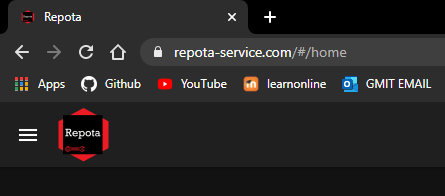
\includegraphics[width=0.8\textwidth]{images/misc/home-route.png}
\end{figure}

\subsubsection{Components \& TypeScript}
Components are controllers for the UI (HTML + SCCS). Components can include various tools for the UI such as forms, buttons, loading in data from an API by the built-in ngOnInit method and navigation. Angular uses TypeScript to turn TypeScript's classes into components. TypeScript by itself cannot compile. It has to be generated and then complied with JavaScript to run. This may ask the question, "Why TypeScript? and not JavaScript?". TypeScript's compiler can catch errors/bugs in advance where as JavaScript only notifies them once it is compiled and running. With TypeScript, errors can be avoided for a production build of an app. TypeScript is built off JavaScript, meaning that JavaScript code can be written in TypeScript with no changes. TypeScript is also quite object-oriented, allowing interfaces to define types for data object models. \cite{ref16}

\subsubsection{ngIf \& ngFor}
Angular uses ngIf as an if statement that can be used across DOMS (Document Body Object). For example, a ngIf can be used if a button on the UI is clicked to load data. ngFor is used as a for loop on the DOM that can loop through arrays of data to avoid DRY code (Don't Repeat Yourself). Meaning that data types can be declared in one HTML div or an Ionic item tag to present multiple data elements on the UI.

\subsection{How Angular \& Ionic fitted the Front-end}
Before this project, Angular and Ionic frameworks have proven to be successful in creating apps for other modules and personal interests. The frameworks with their modules and routing helped to provide smooth navigation throughout the app for users using buttons and a hamburger menu. While the component/page structure allowed the controllers, HTML, and SCCS to be sufficiently organized throughout the entire front-end. ngFor is used throughout the front-end to present data on the UI from the back-end from the ngOnInit methods. ngIf is also used throughout to disable features for unauthorized users and to display messages to users.
Ionic proved to be very useful as it immensely helped make the front-end responsive for mobile phones using the mobile phone simulator Ionic Lab.

\section{MySQL}
MySQL uses the ACID model in its database management system for relational databases (RDBMS). It is the most common open-source database in the world because it is efficient, simple to set up and use. \cite{ref17}  In addition, MySQL is quite robust, both in its setup for database tables and its functionality.
 
\subsection{Relational}
Relational can reduce duplication and redundancy within databases. Rather than storing all of the data in one big storeroom, RDBMS stores it in individual and different tables. Physical files are used to organize the database structures, which are designed for pace. The logical model provides a versatile programming environment with artifacts such as databases, tables to organize data, rows, and columns to separate the data inside tables. \cite{ref18}
 
\subsection{ACID}
The ACID model stands for the database design principles; Atomicity, Consistency, Isolation and Durability. Atomicity is used in InnoDB transactions with statements including 'COMMIT' and 'ROLLBACK'. Transactions are a way of inserting into/updating multiple tables at one time (Figure 3.10). When two tables are linked by foreign keys, transactions are typically used. Consistency protects data from crashes by having transactions broken down into parts. When several transactions are making adjustments and running queries simultaneously, Isolation fine-tunes the balance between efficiency and reliability, accuracy, and reproducibility of results. Finally, Durability which, stores only the successful transactions in the database. \cite{ref19}
 
 \begin{figure}[H]
    \caption{MySQL InnoDB Transaction for inserting data into two tables.}
    \label{image:transaction}
    \centering
    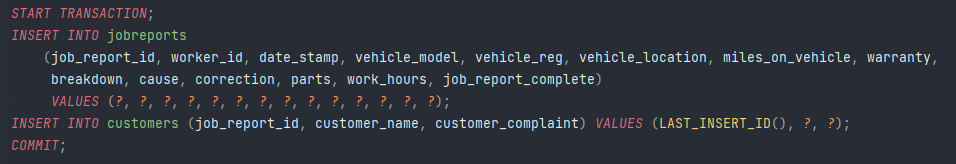
\includegraphics[width=1.0\textwidth]{images/misc/mysql-transation.png}
\end{figure}

\subsection{How MySQL fitted the Database}
MySQL was chosen for many reasons. MySQL definitely seemed like the best fit. As discussed in the introduction, Repota is designed for automobile technicians (workers). In a database, workers need their own dedicated table. For any app, website, system for a company of any sort, there needs to be storage for their workers. If the data were all in one place, it would be a mess, and worker information would get lost right in the middle of it. Having separate, connected tables for data was a necessity for the project. Workers are stored in one table. That table then connects to the service reports table which, is then connected to the customers' table. Keeping dedicated tables for workers and customers was seen as a must as their information if very important for the service reports.

Given that the reports consist of report and customer information, transactions are perfect to create new reports without hassle. MySQL 'JOIN QUERIES' allow selecting data from multiple tables to present the data as if all the data was originally in one table. Since the complete reports consist of data from two other tables, JOIN QUERIES were the way to go. From these observations, it was quite obvious, MySQL was perfect for the database. 

\section{Amazon Web Services}
AWS (Amazon Web Services) is a cloud platform that offers a variety of services. Some of these services are EC2, Route 53, Machine Learning, Elastic Beanstalk, S3 Bucket, Amplify and CloudFront. Deploying to AWS can be as simple as uploading source code files. AWS has its own CLI which, generally works better for deployment. Uploading files can overload the service. Should a significant update needed to be deployed, previous files would first need to be deleted before uploading any new files. With AWS's CLI, command modifiers such as '--delete' can be used during deployment. This modifier deletes any files and deploys the updated ones with ease.

\subsection{Virtual Machines}
Virtual Machines (VM) are virtual emulations of computer environments. \cite{ref20} For example, VMs allow having a Linux Operating System (OS) accessible from the CLI of a Windows computer with no installation needed. From the Windows side, the connection is generally made in a PowerShell or GIT Bash CLI. AWS's EC2 (Elastic Compute Cloud) service handles VMs as instances. EC2 provides the service to have many VMs with different operating systems.

\subsubsection{Windows VS Linux}
Since Window's OS is a commercial product, only the developers who developed it have the authority to alter it. The Linux OS is open-source, allowing users to configure their environments to their taste. Linux is considered to be faster than the most recent Windows versions. Linux is extremely stable because it is simple to find and repair bugs, and in contrast, Windows is vulnerable to viruses and malware because of its vast user base. \cite{ref21}

\subsection{S3 Bucket}
S3 (Simple Storage Service) provides object storage. Objects are the fundamental entities stored in S3. With S3 Bucket, web apps can be stored and hosted. To deploy/upload to a Bucket source code files can be upload or with the AWS CLI. \cite{ref22} By default, these Buckets are HTTP, meaning they are not secure for data transfers. Buckets can become secure (HTTPS) using AWS's Route 53, Certificate Manager, and CloudFront. Route 53 allows to setup hosted zones for a custom web domain. Route 53 takes a domain and routes it to an AWS service such as a S3 Bucket or an Elastic Beanstalk. With CloudFront, that custom domain can become secure. Certificate Manager can issue SSL (Secure Sockets Layer) certificates to domains. That SSL certificate can then be set up with CloudFront. From here, Route 53 can then be used to point the Bucket to the secure CloudFront domain.

\subsection{Elastic Beanstalk}
Elastic Beanstalk (EB) is a service for the deployment and scaling of web apps and services. These web apps and services are usually developed in Java, Ruby, .NET, PHP, Node.js Python, Go and Docker. \cite{ref23} Docker can be used through EB. The addition of Docker and the EB CLI makes deploying to EB a satisfying process. For deployment to EB with Docker, all that is required is a Dockerfile. When deploying to EB with its CLI, it can pick up a Dockerfile in a source code's directory. In deployment, the Dockerfile copies over the source code and pushes it to EB to host. Similar to S3 Buckets EBs are HTTP by default. HTTP can be overcome with a somewhat similar approach to creating a secure Bucket. In the EB configuration settings, a load balancer can be set up to be on a HTTPS port with a SSL certificate. Then Route 53 can be used to point a custom domain to that EB. EB uses Environments to host web apps. These environments have logs to access console outputs, warnings, or information from the web app.

\subsubsection{Docker}
Docker is a series of PaaS (Platform as a Service) products that deliver applications and in 'containers,' as Docker calls them, using OS-level virtual machines. A container is a software packaging file format that encapsulates all of an application's source code and dependencies in a single format that allows it to run easily and efficiently across multiple computing environments. \cite{ref24}

\subsection{How AWS fitted the project's hosting}
AWS seemed like the best fit for hosting as it manages its services very well. The UI itself is well structured and easy to navigate for a cloud platform with several services. The project's database needed to be on a secure server. AWS's EC2 service was opted for the database, hosted on a secure Ubuntu VM. Initially, the project's back-end was also hosted on this VM for prototyping reasons. When the back-end's structure was finalized, it was deployed to EB through Docker. Once the front-end had its core functionality, it was hosted through AWS's S3 Bucket. The back-end and front-end are both HTTPS thanks to AWS's Route 53, CloudFront and Certificate Manager.

